\section{Introduction}
\label{sec:intro}
An established quantized language-model deployment supplies a numerical reference: prompt processing creates its key--value (KV) state, and continuation produces its target vectors and tokens. A prompt provides many known query rows; speculative decoding proposes several continuation tokens for one target verification~\cite{leviathan2023,chen2023}. The optimization problem is to process this known-query work faster while preserving the outputs and state on which regression tests and stateful continuations depend.

A four-query Llama execution illustrates the difficulty (Fig.~\ref{fig:extent_intervention}). Its single-query reference consumed physical KV extents of 768, 768, 768 and 1024 entries; the wider call consumed 1024 for every query. Visible attention inputs and probability prefixes agreed, and the added probabilities were exactly zero, yet the attention output differed. Cropped and padded native replays reproduced the two results. Target vectors diverged before emitted tokens did. Matching the model, positions and causal mask therefore does not determine the runtime's numerical computation.

\begin{figure*}[t]
\centering
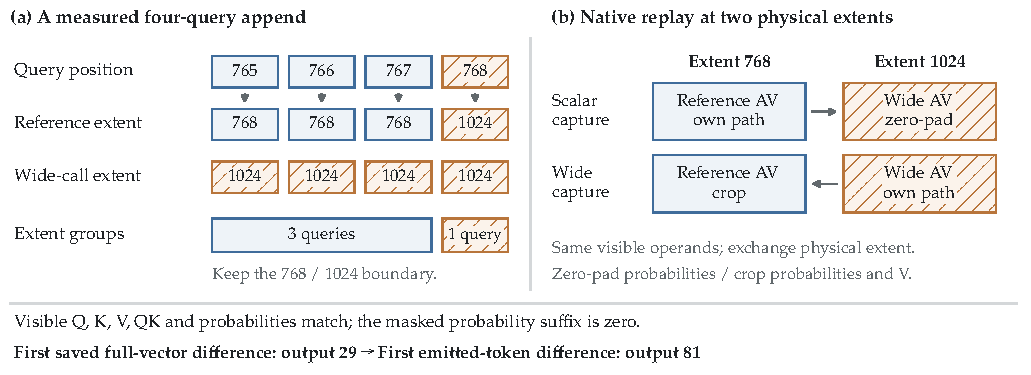
\includegraphics[width=\textwidth]{figures/extent_intervention.pdf}
\caption{Physical-range intervention on the CUDA Llama failure. The four queries require reference extents $[768,768,768,1024]$, while the unsplit call uses 1024. Replays of the first affected query exchange the cropped and padded attention--value (AV) ranges with the consumer query width fixed. The outputs follow the physical range despite identical visible operands and an exactly zero masked probability suffix. The first full-vector discrepancy precedes the first emitted-token discrepancy.}
\label{fig:extent_intervention}
\end{figure*}

Further native interventions identify width-dependent activation quantization, reduction organization and CPU/GPU placement. Producer and commit-state studies show how these requirements extend across calls: compatible arithmetic needs compatible incoming state, and its resulting vectors must remain associated with the retained logical prefix.

We construct a \emph{reference-derived phase plan} from a backend arithmetic recipe and live cache geometry. Source analysis and native operand replays establish the recipe offline. At each call, the planner reads occupancy, physical head, capacity and padding to assign each query its reference extent, then groups adjacent queries with compatible requirements. Whole-graph execution places cuts around the complete computation; local execution confines them to attention and keeps projection and feed-forward work wider. Whole execution also provides the strong simple control for evaluating local cuts.

A separate choice exposes projection parallelism. On the affected CUDA Q8 path, independent groups retain the native four-column computation and run as channels of one GPU operation. A mixed Q4\_K/Q6\_K extension uses scalar-column arithmetic instead. These arithmetic groups differ from the query groups defined by physical KV extent. The executor owns requested outputs by logical row and maintains the committed frontier on one resident target/KV state. Prefill, continuation and verification share this interface while retaining their phase-specific numerical behavior.

Batch-invariant operators control reduction choices~\cite{thinkingmachines}; arithmetic reconstruction and compiler enforcement preserve existing library behavior~\cite{taming}; deterministic engines connect kernel properties with state invariants~\cite{vosti}. Fixed-shape schedules and verified speculation provide system designs for consistent execution~\cite{corun,llm42}. We connect these numerical concerns to a quantized deployment's physical cache range and phase state to determine where known-query work can be combined.

The evaluation first checks full target vectors and active state, then separates the effects of cut placement and arithmetic packing. The implementations cover CUDA and Vulkan, three model families and a 32B mixed-quantization path. In balanced Linux/A5000 experiments, Q8 packing contributes 0.80\%--1.64\%; the contribution of local cuts is smaller because most natural verification calls do not cross a physical boundary. Compatible speculative applications reduce resident service time by 17.21\%, 25.54\% and 11.52\% for Qwen3-8B, Qwen3-14B and Llama-8B against their fastest measured fixed target-only controls. Those application gains include speculation itself. Equal-work and live-request experiments further show why a cheaper wider target call can still produce a slower request when it induces more draft and verification work.

The paper makes two contributions: native interventions identify the physical, arithmetic and state requirements of wider execution, and an execution method derives query cuts, parallelizes independent arithmetic groups and composes calls through explicit output and state ownership. Numerical validation and controlled service measurements evaluate the resulting implementation.
